\section{Datasets}\label{sec:datasets}
Several corpora for LI have been published in the past years. The following list provides an overview of some of the most popular datasets.

\begin{itemize}
    \item \textbf{WiLI-2018:} The Wikipedia language identification dataset is a benchmark dataset designed for written language identification tasks. Introduced by Martin Thoma in 2018, it consists of 1,000 short texts for each of 235 languages, sourced from Wikipedia. The dataset includes a diverse range of languages, covering different writing systems and linguistic families. \cite{Thoma2018}
    \item \textbf{LTI LangID:} Large-scale dataset for language identification, covering over 1,266 languages with text data from diverse sources. It has been instrumental in training models for identifying both high- and low-resource languages. The dataset is particularly valuable for handling noisy, real-world text, making it a key resource for multilingual NLP research. \cite{Caswell2020}
    \item \textbf{Tatoeba:} Free collection of example sentences with translations designed to assist language learners. It is available in over 400 languages. The name "Tatoeba" is derived from Japanese, meaning "for example." The project is maintained by a community of volunteers through open collaboration, and its contributors are known as Tatoebans. \cite{Tatoeba2025}
    \item \textbf{OpenLID:} Introduced by Burchell et al. in 2023, is a curated resource designed to enhance LID across 201 languages. This dataset comprises monolingual text from diverse sources, including news articles, Wikipedia entries, religious texts, and more. To ensure data reliability, the authors conducted a manual audit of samples from each language and source. Both the dataset and the trained model are publicly available, providing valuable resources for the research community. \cite{Burchell2023}
    \item \textbf{LCC:} The Leipzig Corpora Collection is a multilingual corpus repository that includes a wide range of text data in over 200 languages. The collection is maintained by the Natural Language Processing Group at Leipzig University and is freely available for research purposes. The LCC is a valuable resource for training and evaluating language identification models. \cite{Goldhahn2012}
\end{itemize}

\subsection{Khan's WiLI-2018 subset}\label{subsec:wili2018}
The dataset used in this project is a subset of the WiLI-2018 dataset, focusing on a smaller number of languages. This subset includes 22 languages with 1,000 samples each, resulting in a total of 22,000 samples. The text length distribution is shown in \cref{fig:text_length_distribution}. The majority of texts fall between 100 and 500 characters, averaging around 350 characters.

\begin{figure}
    \centering
    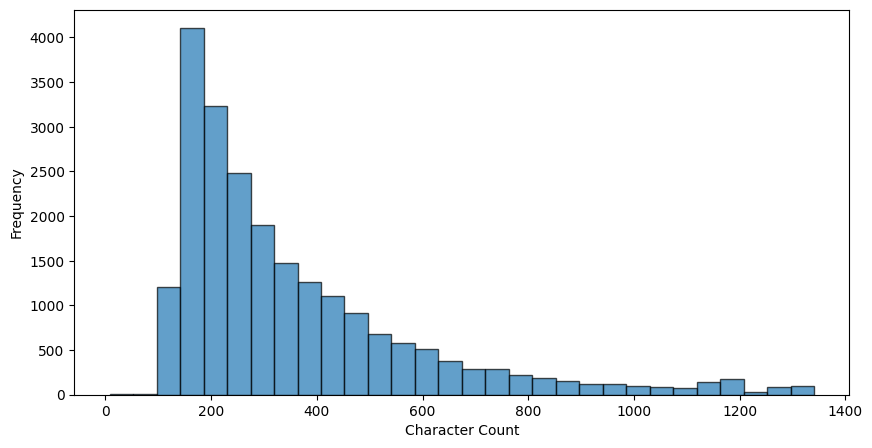
\includegraphics[width=0.8\textwidth]{figures/text_lengths.png}
    \caption{Text length distribution of the WiLI-2018 subset}
    \label{fig:text_length_distribution}
\end{figure}

A closer examination of the texts revealed 141 duplicate entries and one empty text. The duplicates are similarly present in the original dataset and were therefore retained, but the empty text appears to be a newly introduced error in the subset. The empty text was removed from the dataset. It likely originated from preprocessing, where the text was lowercased, and some noise removal was applied. However, the specifics are not disclosed by Khan, the author of the dataset on Kaggle. \cite{Khan2018}

While only a small fraction of the subset exactly matches the texts of the original (2.6\%), the majority (83.4\%) has a high similarity score (> 0.9) with the WiLI-2018 dataset. Similarity was measured using cosine similarity of TF-IDF vectors. 
